%%%%%%%%%%%%%%%%%%%%%%%%%%%%%%%%%%%%%%%%%
% "ModernCV" CV and Cover Letter
% LaTeX Template
% Version 1.1 (9/12/12)
%
% This template has been downloaded from:
% http://www.LaTeXTemplates.com
%
% Original author:
% Xavier Danaux (xdanaux@gmail.com)
%
% License:
% CC BY-NC-SA 3.0 (http://creativecommons.org/licenses/by-nc-sa/3.0/)
%
% Important note:
% This template requires the moderncv.cls and .sty files to be in the same
% directory as this .tex file. These files provide the resume style and themes
% used for structuring the document.
%
%%%%%%%%%%%%%%%%%%%%%%%%%%%%%%%%%%%%%%%%%

%----------------------------------------------------------------------------------------
%	PACKAGES AND OTHER DOCUMENT CONFIGURATIONS
%----------------------------------------------------------------------------------------

\documentclass[11pt,a4paper,sans]{moderncv} % Font sizes: 10, 11, or 12; paper sizes: a4paper, letterpaper, a5paper, legalpaper, executivepaper or landscape; font families: sans or roman

\usepackage[utf8]{inputenc}
\usepackage[english,french]{babel}
\usepackage[T1]{fontenc}
\usepackage{wrapfig}

\moderncvstyle{classic} % CV theme - options include: 'casual' (default), 'classic', 'oldstyle' and 'banking'
\moderncvcolor{blue} % CV color - options include: 'blue' (default), 'orange', 'green', 'red', 'purple', 'grey' and 'black'

% \usepackage{lipsum} % Used for inserting dummy 'Lorem ipsum' text into the template

% \usepackage[scale=0.90]{geometry} % Reduce document margins
\usepackage[height=0.905\paperheight, width=1.37\linewidth]{geometry}
%\setlength{\hintscolumnwidth}{3cm} % Uncomment to change the width of the dates column
%\setlength{\makecvtitlenamewidth}{10cm} % For the 'classic' style, uncomment to adjust the width of the space allocated to your name

\usepackage{color}

\newenvironment{myfont}{\fontfamily{ptm}\fontsize{13pt}{16pt}\selectfont}{\par}

%----------------------------------------------------------------------------------------
%	NAME AND CONTACT INFORMATION SECTION
%----------------------------------------------------------------------------------------

\firstname{\Huge \qquad Fran\c{c}ois} % Your first name
\familyname{\Huge Thierry} % Your last name

% All information in this block is optional, comment out any lines you don't need
\title{\qquad\quad MEng - MSc - PhD}
\address{1 impasse Antoine Watteau\\}{45650 Saint Jean le Blanc, France}
\mobile{+33 (0)6 75 49 39 28}
%\phone{(000) 111 1112}
%\fax{(000) 111 1113}
\email{francois.thierry90@gmail.com}
\homepage{francois-thierry.github.io}{} % The first argument is the url for the clickable link, the second argument is the url displayed in the template - this allows special characters to be displayed such as the tilde in this example
\extrainfo{26 ans, célibataire}
%\photo[70pt][0.4pt]{pictures/picture} % The first bracket is the picture height, the second is the thickness of the frame around the picture (0pt for no frame)

%----------------------------------------------------------------------------------------

\begin{document}

~\

\begin{wrapfigure}{l}{25pt}
  \centering
  \vspace{-2.6cm}
  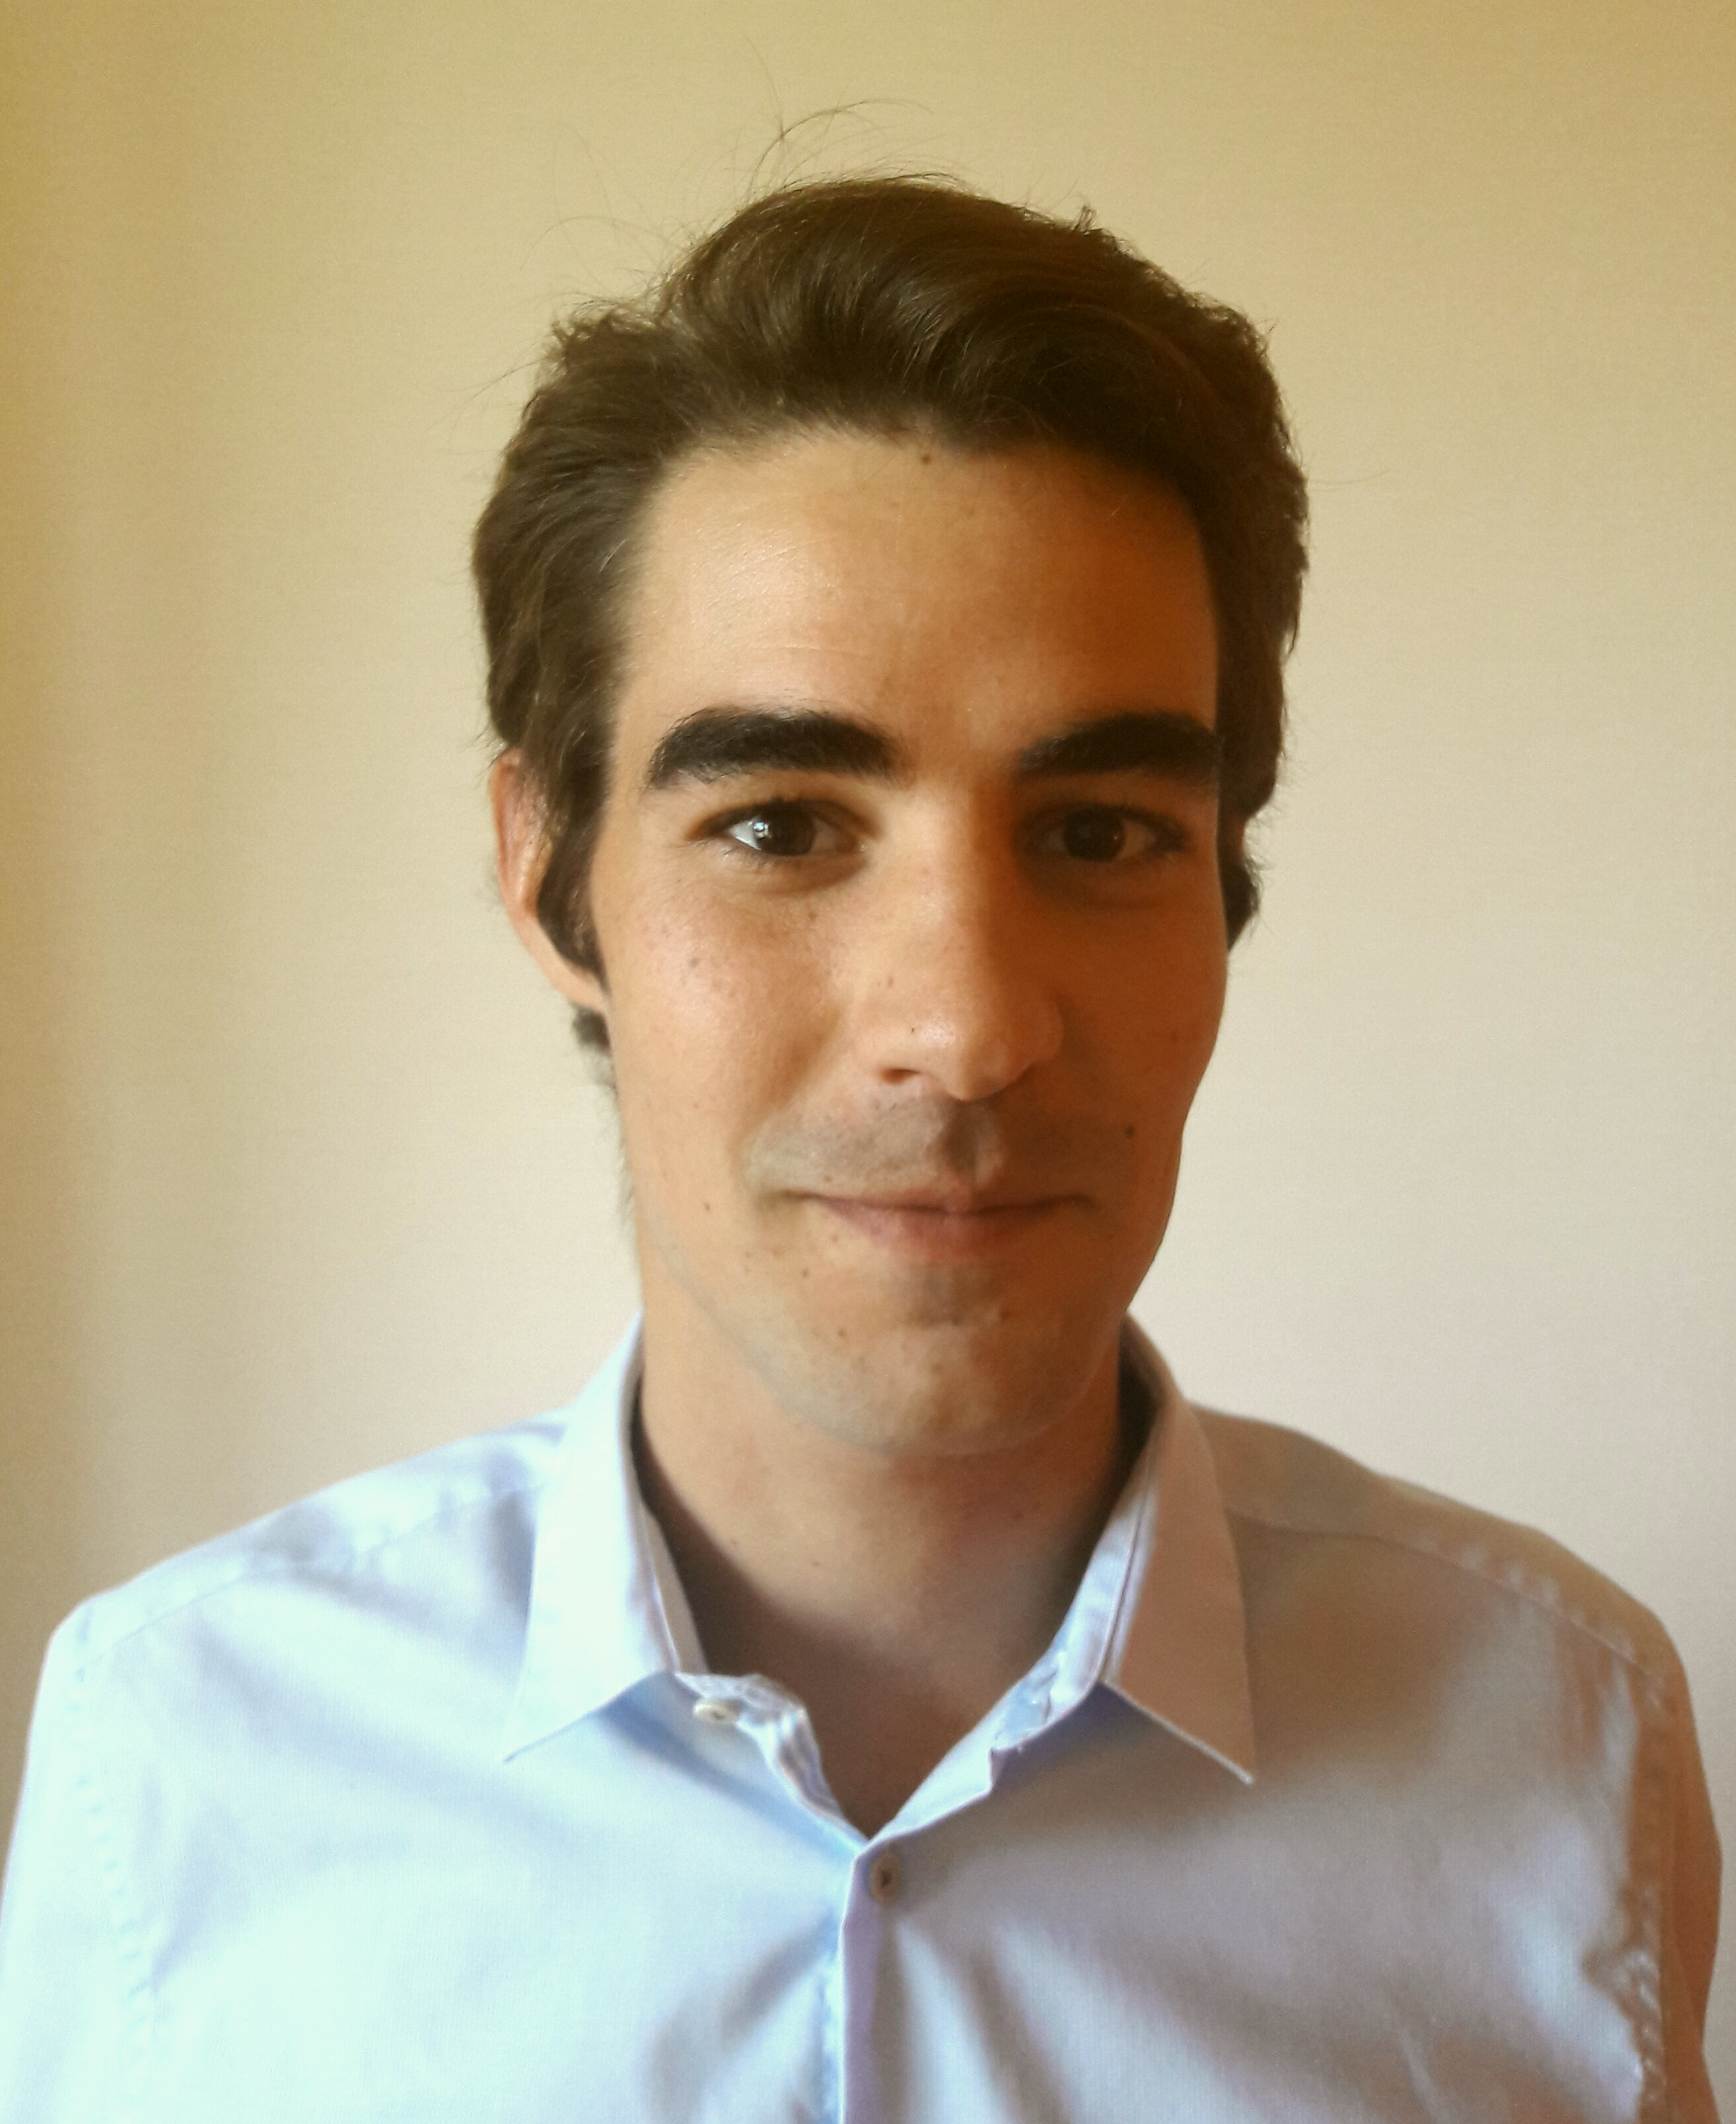
\includegraphics[height=75pt]{photo.png}
  \hfill\vfill
\end{wrapfigure}

~\
\makecvtitle % Print the CV title e

\vspace{-0.7cm}

\cvitem{\bfseries{Mots-cl\'es} :\hfill}{mat\'eriaux, nanosciences, optoélectronique, mod\'elisation, optimisation}{}
%----------------------------------------------------------------------------------------
%	DOCTORAT
%----------------------------------------------------------------------------------------
~\
\section{Doctorat}
\vspace{0.2cm}

\cvitem{2012--2015}{\emph{\bfseries\underline{Titre}: Etude des Propri\'et\'es de Nanoparticules Semiconductrices pour les
Cellules Solaires Hybrides}}
\cvitem{Description}{\textbf{Th\`ese minist\'erielle avec mission d'enseignement} au sein de l'Institut Mat\'eriaux Micro\'electronique Nanosciences de Provence (IM2NP - \textsc{Marseille}) dans l'\'equipe Opto\'electronique et Photovolta\"ique (OPTOPV). Les points clés de ce travail sont:
\begin{itemize}
\item Calcul des propri\'et\'es physiques de structures quantiques
\item Caract\'erisations de couches minces organiques incorporant des nanoparticules
\item Participation à de nombreux projets d'étude numérique de structures optoélectroniques
\end{itemize}
}

%----------------------------------------------------------------------------------------
%	EXPERIENCES PROFESSIONNELLES
%----------------------------------------------------------------------------------------

\section{Exp\'eriences Professionnelles}
\vspace{0.2cm}

\subsection{Stage de recherche - 6 mois}
\cventry{Janvier 2013 Juillet 2013}{\textsc{Universit\'e Leopold-Franzens}}{\textsc{Innsbr\"uck} (Autriche)}{\'equipe photonique}{}{\textbf{Etude des fondements de la physique quantique avec des sources de photon unique}
\begin{itemize}
\item Test de la loi de Born sur des figures d'interf\'erences \`a 3 puis 5 fentes
\item Utilisation de deux sources: montage d'une source optique de photon unique (cristal non lin\'eaire) et utilisation de bo\^ite quantique isol\'ee
\end{itemize}
}
~\
\newline{}

\subsection{Stage R$\&$D - 6 mois}
\cventry{Ao\^ut 2010 F\'evrier 2011}{\textsc{Fraunhofer IPM}}{\textsc{Kaiserslautern} (Allemagne)}{\'equipe mesures et syst\`emes t\'erahertz}{}{\textbf{Caract\'erisation et optimisation d'un nouveau syst\`eme t\'erahertz tout \'electronique}
\begin{itemize}
\item Utilisation et optimisation du nouveau syst\'eme THz d'imagerie non destructive
\item D\'eveloppement d'un logiciel de traitement d'image hyperfr\'equentielles (Matlab)
\end{itemize}
}
~\
\newline{}

\subsection{Stage R$\&$D - 3 mois}
\cventry{Avril 2009 Juillet 2009}{\textsc{LERM}}{\textsc{Arles}}{laboratoire de physique des mat\'eriaux}{}{\textbf{Etude des indicateurs de durabilit\'e des b\'etons et mise en place d'une
nouvelle m\'ethode d'essais par perm\'eabilit\'e \`a l'eau}
\begin{itemize}
\item Caract\'erisation et \'etude de durabilit\'e de nombreux \'echantillons
\item Utilisation et caract\'erisation de la nouvelle m\'ethode d'essai
\end{itemize}
}

~\
\newline{}
% \subsection{Stage R$\&$D - 3 mois}
% \cventry{Et\'e 2005}{\textsc{Centre for Molecular and Nanoscale Electronics}}{\textsc{Durham} (Angleterre)}{}{}{\textbf{Synth�se et caract�risation de nanocomposites}
% }

%----------------------------------------------------------------------------------------
%	EDUCATION SECTION
%----------------------------------------------------------------------------------------
\section{Formation}
\vspace{0.2cm}

% \cventry{2003--2006}{Ing�nieur G�nie Physique}{Polytech' Clermont-Ferrand (Ex. CUST)}{\textsc{Clermont-Ferrand}}{}{Sp�cialisation en Science des Mat�riaux}  % Arguments not required can be left empty
\cventry{2011--2012}{Master en Sciences, Technologies \& Sant\'e}{Mention M\'ecanique et Physique Sp\'ecialit\'e Optique et Nanotechnologies (ONT)}{\textsc{Universit\'e de Technologie de Troyes (UTT)}}{}{}
\cventry{2009--2012}{Formation Ing\'enieur}{Mention Mat\'eriaux, Technologie et Economie (MTE) Sp\'ecialit\'e Transformation et Qualit\'e des Mat\'eriaux (TQM)}{\textsc{Universit\'e de Technologie de Troyes}}{}{}
\cventry{2007--2009}{DUT}{en Science et G\'enie des Mat\'eriaux}{\textsc{Universit\'e Fran\c{c}ois Rabelais de Tours}}{\newline\textsc{IUT de Blois}}{}

%----------------------------------------------------------------------------------------
%	COMMUNICATION SKILLS SECTION
%----------------------------------------------------------------------------------------

~\
\vspace{-0.2cm}
\section{Publications et Communications}

\cvitem{}{
Les articles sont téléchargables sur \href{https://www.researchgate.net/profile/Francois_Thierry}{\bfseries ResearchGate} et \href{https://github.com/Francois-Thierry/about-me/tree/master/publications}{\bfseries GitHub}
}
\vspace{0.3cm}
%
\cvitem{2016}{ -
J. Le Rouzo, D. Duché, C. Ruiz-Herrero, {\bfseries F. Thierry}, M. Carlberg, G. Berginc, M. Pasquinelli, J-J. Simon, L. Escoubas, and F. Flory,
"Specific tools for studying the optical response of heterogeneous thin film layers", Journal of Nanophotonics - soumis
}
\cvitem{}{ -
J. Le Rouzo, D. Duch\'e, C.M. Ruiz, {\bfseries F. Thierry}, M. Carlberg, G. Berginc, M. Pasquinelli, J.J. Simon, L. Escoubas and F. Flory,
"Characterization and modeling tools for light management in heterogeneous thin film layers", Proceedings of SPIE - The International Society for Optical Engineering 99290I \href{http://dx.doi.org/10.1117/12.2237682}{[lien]}
}
\cvitem{2015}{ -
{\bfseries F. Thierry}, J. Le Rouzo, F. Flory, G. Berginc and L. Escoubas,
"Fast and reliable approach to calculate energy levels in semiconductor nanostructures", Journal of Nanophotonics, 9(1), 093080. \href{http://dx.doi.org/10.1117/1.JNP.9.093080}{[lien]}
}
\cvitem{2014}{ -
A. Bou, P. Torchio, D. Barakel, {\bfseries F. Thierry}, A. Sangar, P-Y. Thoulon and M. Ricci, "Indium tin oxide-free transparent and conductive electrode based on SnOx | Ag | SnOx for organic solar cells", Journal of Applied Physics, 116, 023105 \href{http://dx.doi.org/10.1063/1.4886225}{[lien]}
}
\cvitem{}{ -
{\bfseries F. Thierry}, J. Le Rouzo, F. Flory, G. Berginc and L. Escoubas, "Optimization of the optical properties of nanostructures through fast numerical approaches", Proceedings of SPIE - The International Society for Optical Engineering 916102 \href{http://dx.doi.org/10.1117/12.2061042}{[lien]}
}
\cvitem{}{ -
A. Bou, P. Torchio, D. Barakel, {\bfseries F. Thierry}, P-Y. Thoulon and M. Ricci,  "Numerical and experimental study of SnOx | Ag | SnOx multilayer as indium-free transparent electrode for organic solar cells", Proceedings of SPIE - The International Society for Optical Engineering 898706 \href{http://dx.doi.org/10.1117/12.2039067}{[lien]}
}

%----------------------------------------------------------------------------------------
%	AWARDS SECTION
%----------------------------------------------------------------------------------------
~\
\newline{}
\section{Prix et Distinctions}

~\

\cvitem{2014}{ - Newport Research Excellence Award - SPIE Optics + Photonics, San Diego, USA}
\cvitem{}{ - Prix du meilleur poster de th\`ese 2$^{\mathrm{\`eme}}$ ann\'ee - Journ\'ees de l'IM2NP, Cassis, France}

%----------------------------------------------------------------------------------------
%	COMPUTER SKILLS SECTION
%----------------------------------------------------------------------------------------
~\
\section{Comp\'etences Informatique}

~\

\cvitem{Programmation}{{\bfseries Python}, C/C++, HTML/Javascript, Matlab}
\cvitem{Bureautique}{{\bfseries \LaTeX}, Microsoft Office, Reveal.js}
\cvitem{Graph./CAO}{{\bfseries Inkscape}, Gimp, Photoshop / Autodesk Inventor}


%----------------------------------------------------------------------------------------
%	LANGUAGES SECTION
%----------------------------------------------------------------------------------------
~\
\section{Langues Pratiqu\'ees}

~\

\cvitem{Fran\c{c}ais}{Langue maternelle}{}
\cvitem{{\bfseries Anglais}}{Courant}{}
\cvitem{{\bfseries Allemand}}{Courant}{}
\cvitem{Espagnol}{Notions}{}
\cvitem{Italien}{Notions}{}

%----------------------------------------------------------------------------------------
%	INTERESTS SECTION
%----------------------------------------------------------------------------------------

%\section{Int�rets}

%\renewcommand{\listitemsymbol}{-~} % Changes the symbol used for lists
%
%\cvlistdoubleitem{Boxe}{Cin�ma}
%\cvlistdoubleitem{Informatique}{M�canique}
%\cvlistdoubleitem{Voyages}{Cin�ma}

%----------------------------------------------------------------------------------------
%	COVER LETTER
%----------------------------------------------------------------------------------------

% To remove the cover letter, comment out this entire block

%\clearpage
%
%\recipient{HR Departmnet}{Corporation\\123 Pleasant Lane\\12345 City, State} % Letter recipient
%\date{\today} % Letter date
%\opening{Dear Sir or Madam,} % Opening greeting
%\closing{Sincerely yours,} % Closing phrase
%\enclosure[Attached]{curriculum vit\ae{}} % List of enclosed documents
%
%\makelettertitle % Print letter title
%
%\lipsum[1-3] % Dummy text
%
%\makeletterclosing % Print letter signature

%----------------------------------------------------------------------------------------

\end{document}
